\documentclass[tikz,border=8pt]{standalone}
\usepackage{amsmath,amssymb,bm}
\usepackage{sansmath}
\usepackage{tikz}
\usetikzlibrary{arrows.meta,calc}
\usepackage{pgfplots}
\pgfplotsset{compat=1.16}
\usepgfplotslibrary{groupplots}
\definecolor{cteal}{HTML}{2F5D62}\definecolor{cred}{HTML}{A44A3F}\definecolor{cochre}{HTML}{B08A45}
\definecolor{cgray}{HTML}{666360}\definecolor{clgray}{HTML}{9A9791}\definecolor{csage}{HTML}{7D9D8C}
\definecolor{cpurple}{HTML}{7A5B78}\definecolor{cdark}{HTML}{3B3A38}\definecolor{cmid}{HTML}{8E8B85}\definecolor{cpaper}{HTML}{F6F4F0}
\pgfplotsset{paper/.style={font=\sffamily\sansmath\scriptsize, axis line style={black!65,line width=0.4pt},
  tick style={black!65,line width=0.4pt}, tick align=outside, major tick length=2pt,
  axis x line*=bottom, axis y line*=left, grid style={line width=0.3pt,black!10},
  legend style={draw=none,fill=none,font=\sffamily\sansmath\scriptsize}, legend cell align=left,
  title style={font=\sffamily\sansmath\scriptsize,at={(0,1)},anchor=south west,yshift=3pt,xshift=-2pt},
  label style={font=\sffamily\sansmath\scriptsize}, ticklabel style={font=\sffamily\sansmath\scriptsize},
  yticklabel style={font=\sffamily\sansmath\scriptsize}, xticklabel style={font=\sffamily\sansmath\scriptsize}}}


\newcommand{\logit}{\operatorname{logit}}\newcommand{\expit}{\operatorname{expit}}
\begin{document}
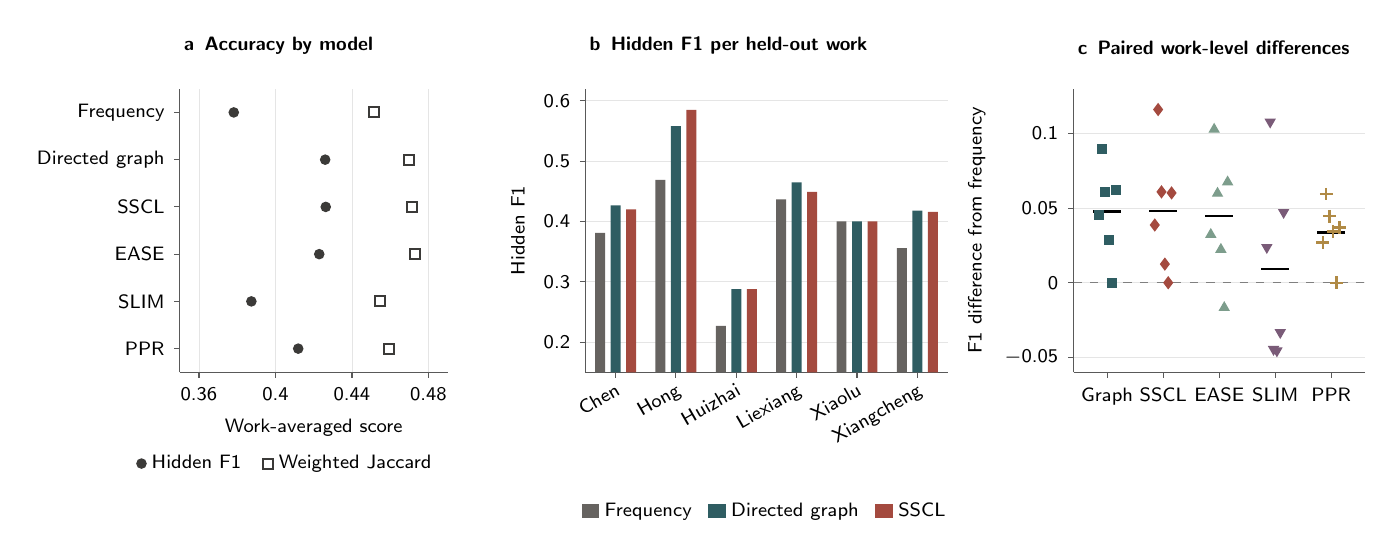
\begin{tikzpicture}
\begin{axis}[paper, at={(1.75cm,0)}, scale only axis, width=3.4cm, height=3.6cm,
  xmin=0.35, xmax=0.49, ymin=0.5, ymax=6.5, ytick={1,...,6},
  yticklabels={PPR,SLIM,EASE,SSCL,Directed graph,Frequency},
  xtick={0.36,0.40,0.44,0.48}, xticklabel style={/pgf/number format/fixed,/pgf/number format/precision=2},
  xlabel={Work-averaged score}, xmajorgrids, title={\textbf{a}\enspace\textbf{Accuracy by model}},
  legend style={at={(0.4,-0.25)},anchor=north,legend columns=2,/tikz/every even column/.append style={column sep=6pt}}]
\addplot[only marks,mark=*,mark size=1.7pt,color=cdark] coordinates {(0.3782,6) (0.4260,5) (0.4263,4) (0.4229,3) (0.3874,2) (0.4119,1)};
\addplot[only marks,mark=square,mark size=1.8pt,draw=cdark,line width=0.7pt] coordinates {(0.4514,6) (0.4699,5) (0.4716,4) (0.4730,3) (0.4545,2) (0.4594,1)};
\legend{Hidden F1,Weighted Jaccard}
\end{axis}
\begin{axis}[paper, at={(6.9cm,0)}, scale only axis, width=4.6cm, height=3.6cm,
  ybar, bar width=3.6pt, ymin=0.15, ymax=0.62, ytick={0.2,0.3,0.4,0.5,0.6},
  yticklabel style={/pgf/number format/fixed,/pgf/number format/precision=1},
  symbolic x coords={Chen,Hong,Huizhai,Liexiang,Xiaolu,Xiangcheng}, xtick=data,
  x tick label style={rotate=30,anchor=north east,inner sep=1pt}, enlarge x limits=0.1,
  ylabel={Hidden F1}, ymajorgrids, title={\textbf{b}\enspace\textbf{Hidden F1 per held-out work}},
  legend style={at={(0.5,-0.42)},anchor=north,legend columns=3,/tikz/every even column/.append style={column sep=4pt}}, legend image code/.code={\draw[#1,draw=none] (0cm,-0.08cm) rectangle (0.22cm,0.1cm);}]
\addplot[fill=cgray,draw=none] coordinates {(Chen,0.3812) (Hong,0.4689) (Huizhai,0.2268) (Liexiang,0.4365) (Xiaolu,0.4000) (Xiangcheng,0.3557)};
\addplot[fill=cteal,draw=none] coordinates {(Chen,0.4268) (Hong,0.5583) (Huizhai,0.2877) (Liexiang,0.4649) (Xiaolu,0.4000) (Xiangcheng,0.4180)};
\addplot[fill=cred,draw=none] coordinates {(Chen,0.4199) (Hong,0.5850) (Huizhai,0.2877) (Liexiang,0.4490) (Xiaolu,0.4000) (Xiangcheng,0.4159)};
\legend{Frequency,Directed graph,SSCL}
\end{axis}
\begin{axis}[paper, at={(13.1cm,0)}, scale only axis, width=3.7cm, height=3.6cm,
  xmin=0.4, xmax=5.6, ymin=-0.06, ymax=0.13, xtick={1,...,5},
  xticklabels={Graph,SSCL,EASE,SLIM,PPR}, ytick={-0.05,0,0.05,0.10},
  yticklabel style={/pgf/number format/fixed,/pgf/number format/precision=2},
  ylabel={F1 difference from frequency}, ymajorgrids, title={\textbf{c}\enspace\textbf{Paired work-level differences}}]
\draw[black!50,dashed] (axis cs:0.4,0)--(axis cs:5.6,0);
\addplot[only marks,mark=square*,mark size=1.6pt,color=cteal] coordinates {(0.85,0.0456) (0.91,0.0894) (0.97,0.0609) (1.03,0.0284) (1.09,0) (1.15,0.0623)};
\addplot[only marks,mark=diamond*,mark size=2.1pt,color=cred] coordinates {(1.85,0.0387) (1.91,0.1161) (1.97,0.0609) (2.03,0.0125) (2.09,0) (2.15,0.0602)};
\addplot[only marks,mark=triangle*,mark size=2pt,color=csage] coordinates {(2.85,0.0323) (2.91,0.1028) (2.97,0.0599) (3.03,0.0223) (3.09,-0.0167) (3.15,0.0675)};
\addplot[only marks,mark=triangle*,mark options={rotate=180},mark size=2pt,color=cpurple] coordinates {(3.85,0.0237) (3.91,0.1078) (3.97,-0.0446) (4.03,-0.0456) (4.09,-0.0333) (4.15,0.0472)};
\addplot[only marks,mark=+,mark size=2.3pt,color=cochre,line width=0.9pt] coordinates {(4.85,0.0269) (4.91,0.0594) (4.97,0.0446) (5.03,0.0345) (5.09,0) (5.15,0.0370)};
\draw[black,line width=1pt] (axis cs:0.75,0.0478)--(axis cs:1.25,0.0478) (axis cs:1.75,0.0481)--(axis cs:2.25,0.0481)
  (axis cs:2.75,0.0447)--(axis cs:3.25,0.0447) (axis cs:3.75,0.0092)--(axis cs:4.25,0.0092) (axis cs:4.75,0.0337)--(axis cs:5.25,0.0337);
\end{axis}
\end{tikzpicture}
\end{document}
